\chapter{粗粒度稀疏神经网络加速器}

深度压缩的神经网络能够减少数据存储需求、计算量、数据传输量,最终提高计算性能,减少计算能耗。\zadd{由于传统的计算平台如CPU和GPU等不能充分利用深度压缩的神经网络的优秀特性,如粗粒度稀疏,量化等;因此我们设计专用的硬件加速器,Cambricon-S,充分挖掘深度压缩神经网络的优秀特性。} Cambricon-S最主要的特征是两个选数逻辑:神经元选择模块 (neuron selector module, NSM) 和突触选择模块(synapse selector module, SSM),分别用来处理静态稀疏和动态稀疏,过滤不必要的神经元和权值,筛选出需要进行计算的神经元和权值。除了两个选数模块,我们设计了WDM(weight decoding module)和Encoder分别支持局部量化和动态压缩神经元。同时,我们设计了一个多发射的控制器,能够同时发射没有依赖关系的指令,从而挖掘IO与计算之间的并行性,进一步提高加速器的性能。


\zadd{本章中我们首先以一个粗粒度稀疏的全连接神经网络为驱动实例,充分分析神经网络加速器的设计原则。然后我们根据这些设计原则设计对应的神经网络加速器。最后我们为加速器设计了一套基于库的编程框架以减轻用户的编程负担。
}

\section{设计原则}
\label{sec:principle}


我们首先使用一个经过粗粒度稀疏的全连接层作为示例(参见图~\ref{fig:connection}),分析粗粒度稀疏神经网络的特性,进而分析出神经网络加速器的设计原则。在图中,我们只关注其中规模为$8\times 3$的部分连接,我们使用$2\times 3$的剪枝块对全连接层进行剪枝。由于粗粒度剪枝,输入神经元$n1, n2$与输出神经元$o1, o2, o3$之间的连接被完全裁剪;输入神经元$n5, n6$与输出神经元$o1, o2, o3$之间的连接也被完全裁剪。由于ReLU激励函数,输入神经元$n4, n6, n8$的激活为“0”。我们采用直接索引的方式标志非零权值的信息,
即我们使用\emph{“00110011”}比特串标志与输出神经元$o1, o2, o3$对应的突触,其中“0”表示对应的突触被裁剪,“1”表示对应的突触存在。
通过观察,我们发现了以下四个粗粒度稀疏神经网络的特性。

\begin{figure}[ht]
\centering
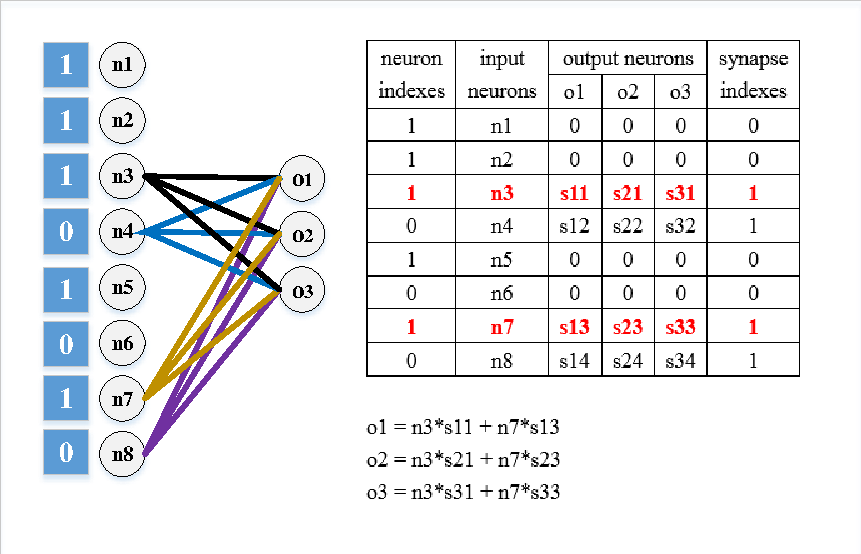
\includegraphics[width=0.8\columnwidth]{connection.pdf}
\caption{粗粒度稀疏的全连接层}
\label{fig:connection}
\end{figure}

首先,多个输出神经元之间共享索引信息。如图~\ref{fig:connection}所示,输入神经元$n1$,$n2$,$n5$, $n6$与输出神经元$o1, o2, o3$之间的连接被同时剪除,因此输出神经元之间共享相同的连接拓扑,也就是说它们共享相同的权值索引表示~\emph{“00110011”}(图中的“Synapse Indexes”)。尽管输出神经元之间不共享相同的权值,但所选权重的位置是相同的,因此是一种部分共享。

第二,多个输出神经元之间共享输入神经元。如图~\ref{fig:connection}所示,最终需要参与计算的神经元是$n3, n7$,它们的值被输出神经元共享。不失一般性,在完全连接的层中,设定修剪块大小为$(B_{in},B_{out})$,那么$B_{out}$个相邻输出神经元将共享相同的输入神经元。在卷积层中,设定剪枝块的大小为为$(B_{fin},B_{fout},B_x,B_y)$,那么$B_{fout}$个相邻的输出神经元将共享相同的输入神经元。

第三,动态稀疏性能够进一步提高运算效率。在图中,通过挖掘权值稀疏,输入神经元$n3, n4, n7, n8$被筛选出来进行计算,同时由于输入神经元$n4, n8$的激活为零,在运算过程中,它们对输出神经元没有贡献,最后需要进行计算的输入神经元为$n3, n7$。在图中的实例中,通过挖掘权值稀疏性,共需要进行12次乘法,9次加法完成运算;同时挖掘权值稀疏性和动态神经元的稀疏性,只需要进行6次乘法和3次加法。对比在稠密情况下24次乘法和21次加法,分别有2.14倍和5倍的性能提升。因此,利用动态神经元稀疏性是进一步提高效率的关键(在上面的示例中,能够进一步提升2倍性能)。值得注意的是,即使考虑到动态神经元稀疏,输出神经元仍然共享索引和所选的输入神经元。

第四,多个输出神经元之间的负载是平衡的,因为它们共享相同的输入神经元。对于图~\ref{fig:connection}中的示例,如果考虑静态稀疏,那么每个输出神经元共享相同的输入神经元$n3, n4, n7, n8$,同时需要四个对应的权值$S_{Ti1}, S_{Ti2}, S_{Ti3}, S_{Ti4}$进行计算,因此每个输出神经元需要进行4次乘法和3次加法完成运算。如果同时考虑静态稀疏和动态稀疏,那么每次输出神经元共享相同的输入神经元$n3, n7$,同时需要两个对应的权值$S_{Ti1}, S_{Ti3}$进行计算,因此每个输出神经元需要进行2次乘法和1次加法完成运算。因此粗粒度稀疏的神经网络可以避免负载不平衡而造成的性能损失~\cite{han2017ese}。

因此,在设计加速器时要考虑以下原则,以最大限度地提高加速器的效率:加速器(1)能够利用共享的索引信息和共享的输入神经元信息,简化加速器的设计;(2)能够利用动态稀疏性进一步提高效率;(3)利用相邻输出神经元之间的负载均衡。


\section{Cambricon-S的架构}
\begin{figure}[h]
\centering
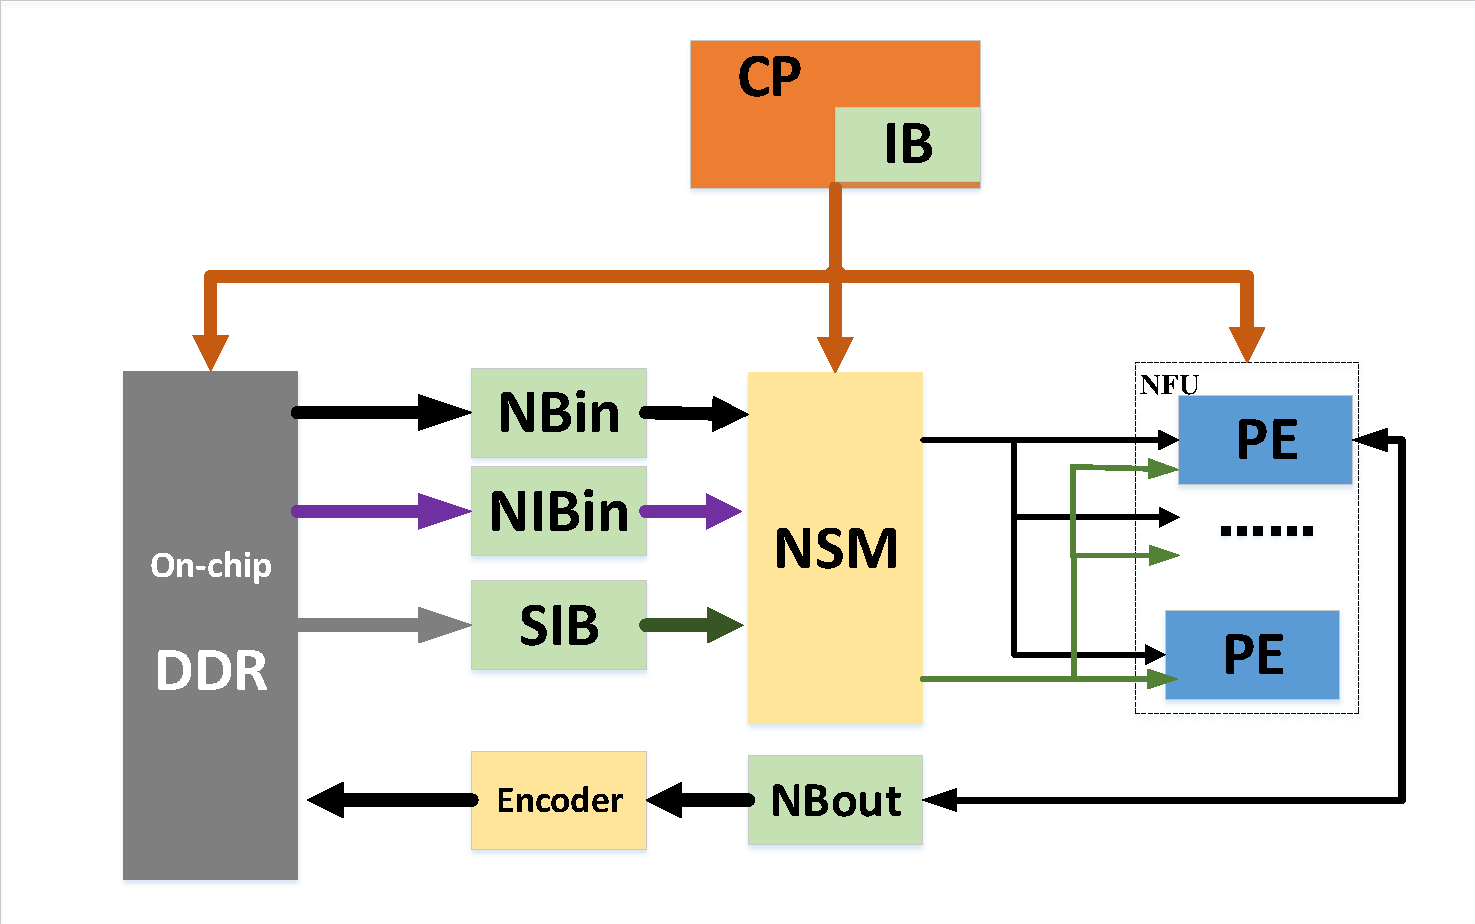
\includegraphics[width=0.8\columnwidth]{ACC.pdf}
\caption{Cambricon-S整体架构}
\label{fig:acc}
\end{figure}

在本节中,我们将介绍Cambricon-S的详细架构,它能够充分利用深度压缩神经网络带来的收益,有效地解决粗粒度修剪稀疏网络的剩余不规则性。

如图~\ref{fig:acc}所示,我们展示了加速器架构。按照~\ref{sec:principle}的设计原则,我们在加速器中设计了一个关键模块-神经元选择器模块(neural selector module, NSM),用于处理静态稀疏和共享信息(包括共享索引信息和共享神经元信息)。同时我们设计了一个神经功能单元(neural functional unit,NFU)用于完成神经网络中的核心计算。NFU中具有多个处理单元(processing elements, PEs)用来并行计算不同的输出神经元。每个PE都包含一个本地的突触选择器模块(synapse selector module, SSM)来处理动态稀疏性。动态神经元压缩模块(Encoder)用于动态地将输出神经元压缩成为非零元素/非零元素索引的模式,从而减少Load/Store神经元的开销。存储模块需要存储输入神经元,权值和输出神经元,因此我们需要输入神经元缓存(input neuron buffer, NBin),输出神经元缓存(output neuron buffer, NBout)和突触缓存(synapse buffer, SB),考虑到神经元和权值的稀疏性,我们需要两个额外的缓存,即输入神经元索引缓存(input neuron index buffer, NIBin)和突触索引缓存(synapse index buffer, SIB )分别存储输入神经元索引和突触索引信息。注意,其中SB被内置与NFU的每一个PE中,没有表现在图中。控制模块由控制处理器(control processor, CP)和指令缓存(instruction buffer, IB)组成,CP有效地将IB中存储的各种指令解码为所有其他模块的详细控制信号,我们将CP设计为一个多发射的控制器(multi-issue controller),从而挖掘访存与计算之间的并行性,进一步提升加速器的性能,同时我们为加速器定义一个VLIW(very long instruction word)风格的指令集。

下面我们将从稀疏处理,存储,控制和片上互联四个方面介绍加速器。

\subsection{稀疏处理}
该加速器旨在利用(1)静态稀疏性和(2)动态稀疏性,以及(3)局部量化,从而减少数据存储量、数据传输量、计算量,进而提升性能,并节约能耗。在加速器中,稀疏性由NSM,NFU和Encoder这三个模块共同处理。NSM接收来自NBin的输入神经元,来自NIBin的输入神经元索引和来自SIB的突触索引,筛选出需要进行计算的神经元(静态稀疏),同时生成筛选突触的突触标志(synapse flags),然后将筛选出的神经元和突触标志通过NFU广播给PE。每个PE中的SSM通过突触标志筛选出需要进行计算的突触(动态稀疏),避免无用的计算和数据传输,提高加速器的性能。Encoder用来动态压缩稀疏的输出神经元,减少片外访存能耗。此外每个PE中集成了一个权值解码模块(WDM),用于解码经过局部量化的权值。

\subsubsection{Indexing}
在详细说明NSM,NFU,Encoder之前,我们将详细说明如何在加速器中存储和索引稀疏数据。表示稀疏数据的方法主要有两类,\zadd{分别是二进制掩码(binary mask)和数值索引(numerical indexing)},这两类方法都仅存储非零元素,使用不同的方式索引非零元素。二进制掩码的方式主要包括直接索引(direct indexing),我们使用比特串对非零元素进行索引,其中"0"表示对应的位置的元素为零,"1"表示对应位置元素为非零。数值索引包括步长索引(step indexing),压缩稀疏行(compressed sparse row, CSR),压缩稀疏列(compressed sparse column,CSC),坐标列表查找(coordinate list,COO)等,它们主要使用非零元素之间相对位置(步长)或者绝对位置信息对非零元素进行索引。

由于目前主流的神经网络稀疏度低于$95\%$,采用CSR、CSC、COO等方式的存储开销远远大于直接索引或者步长索引的方式;而且考虑到神经元和突触同时稀疏,步长索引这种方式很难索引到两者同时非零的情况,因此我们采用直接索引的方式存储稀疏神经元和稀疏权值。如图~\ref{fig:connection},我们仅需要存储$n1, n2, n3, n5, n7$这五个神经元和~\emph{“11101010”}比特串就能够表示稀疏的输入神经元;同时我们仅需要存储$s11, s12, s13, s14$这四个权值和~\emph{“00110011”}比特串就能够表示与$o1$相连的稀疏突触。值得注意的是,由于稀疏权值是一种静态稀疏,这种编码压缩过程可以离线完成;但是稀疏神经元是一种动态稀疏,这个过程需要在线实时完成,因此我们需要Encoder模块对稀疏神经元进行动态压缩。

\subsubsection{NSM}
\begin{figure}[h]
\centering
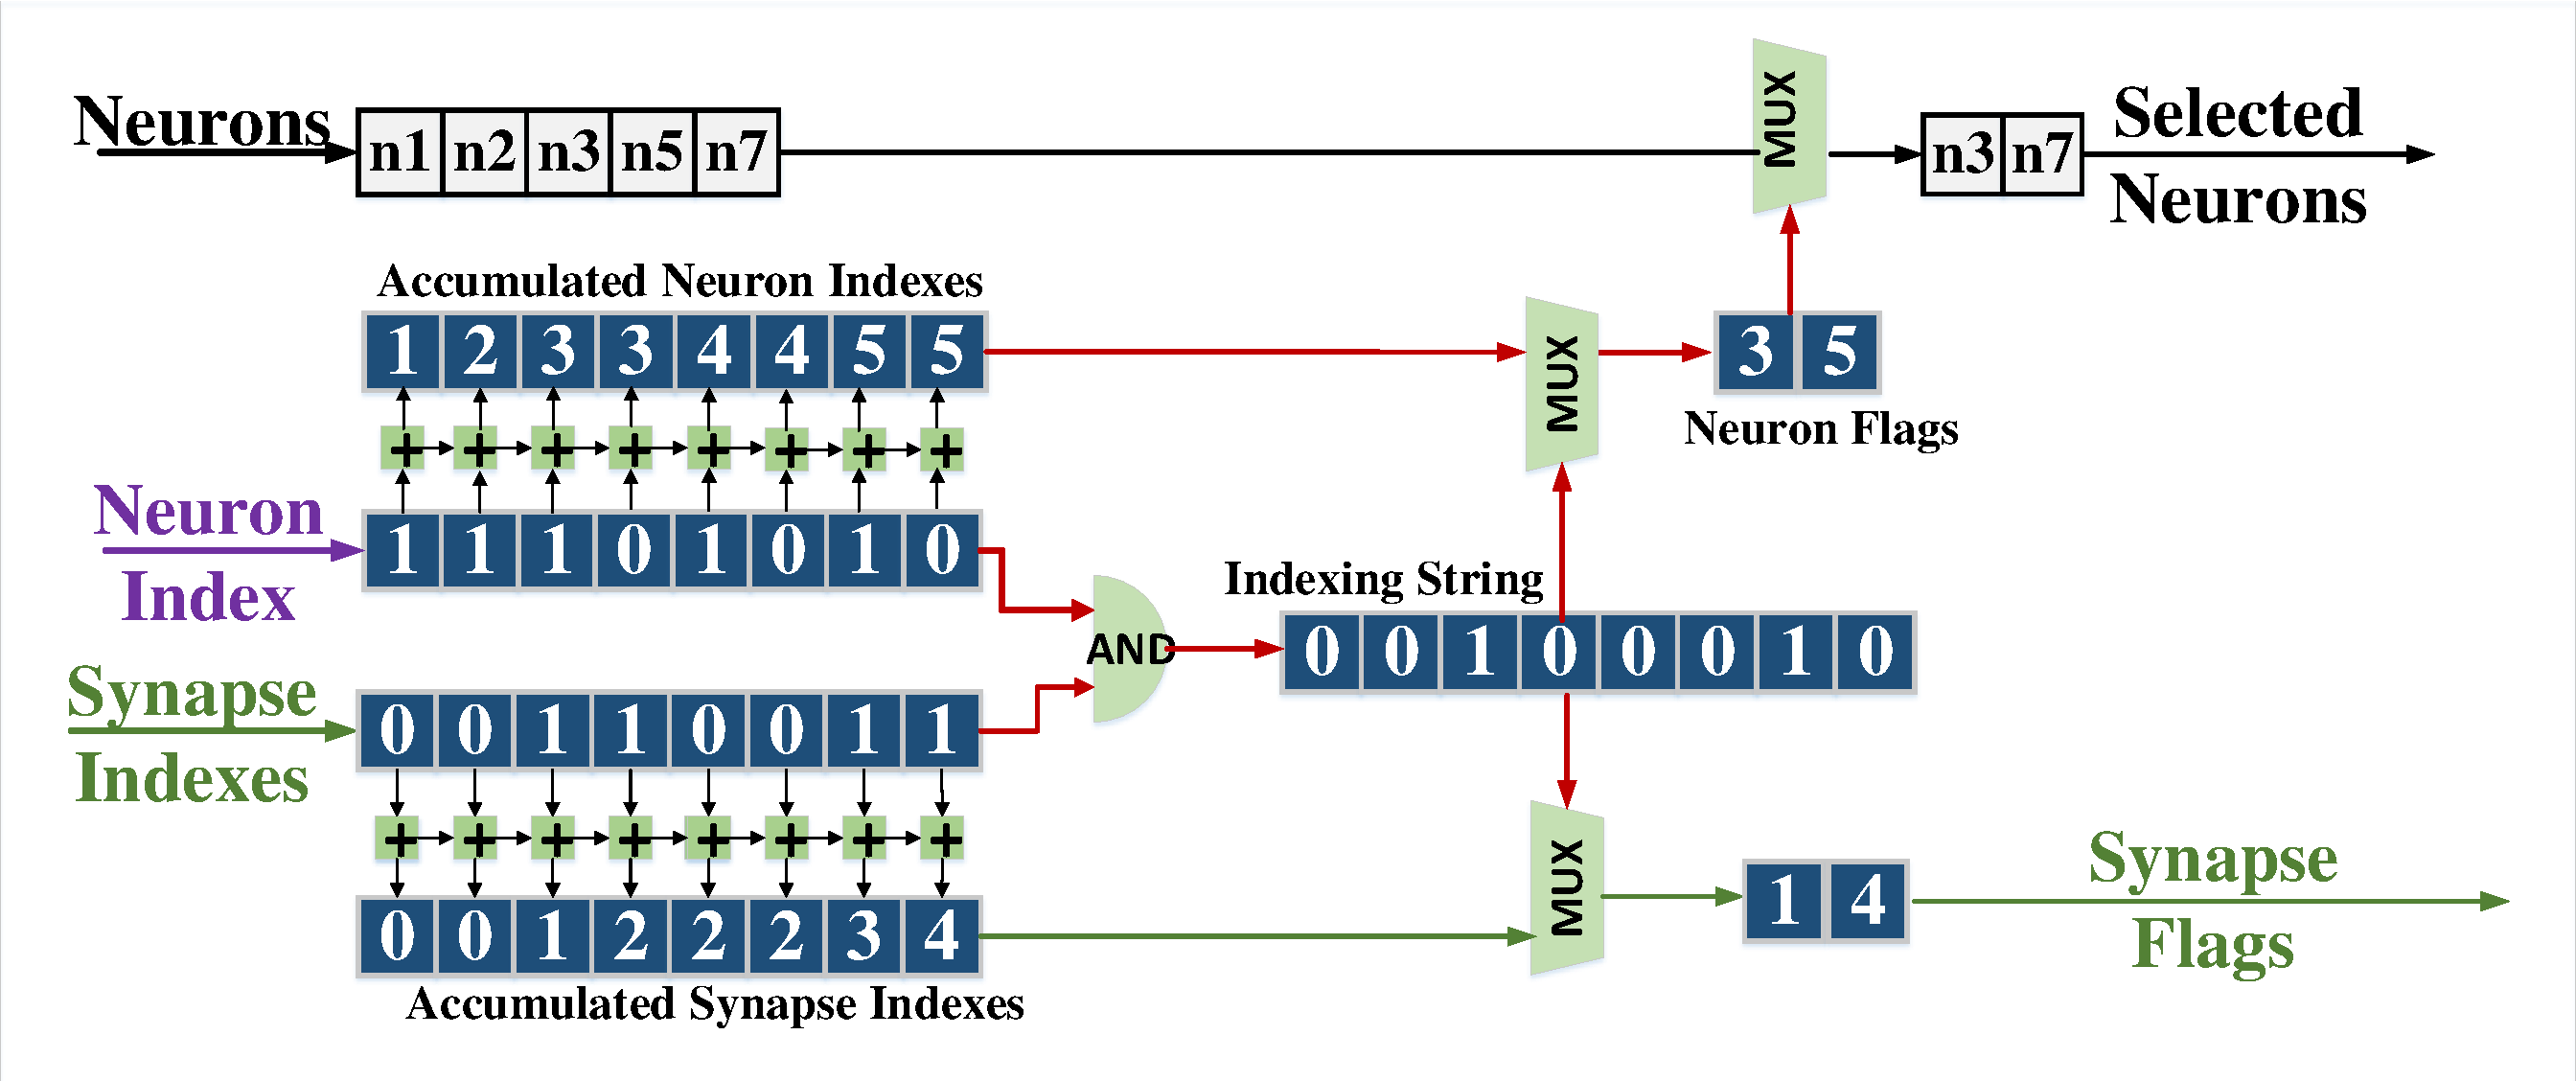
\includegraphics[width=0.8\columnwidth]{NSM.pdf}
\caption{NSM结构}
\label{fig:NSM}
\end{figure}

如图~\ref{fig:NSM}所示,NSM模块的输入为输入神经元,输入神经元索引和突触索引,NSM模块通过神经元索引和突触索引筛选需要进行计算的输入神经元来处理静态稀疏。为了更有效地利用粗粒度稀疏特性,即多个相邻的输出神经元共享索引和输入神经元,我们设计了一个中心NSM,它能够广播筛选出的输入神经元信息到多个PE中,从而完成输入神经元的共享,保证多个PE之间的负载均衡。我们利用图~\ref{fig:connection}作为实例来描述NSM筛选输入神经元的流程。

\zadd{在图~\ref{fig:connection}中的实例中,NSM需要从8个输入神经元中筛选出需要进行计算的神经元$n3, n7$,同时生成筛选突触需要的突触标志(synapse flags,\emph{“14”})。具体来说,首先NSM对神经元索引(neuron indexes,~\emph{“11101010”})和突触索引(synapse indexes,\emph{“00110011”})执行 “AND” 操作,从而生成索引串(indexing string,\emph{“00100010”})。同时神经元索引和突触索引分别累计自身,获得累加神经元索引(accumulated neuron indexes,\emph{“12334455”}) 和累加突触索引(accumulated synapse indexes,\emph{“00122234”}),然后分别与索引串执行 “MUX” 操作,生成神经元标志(neuron flags,\emph{“35”}) 和突触标志 (\emph{“14”})。神经元标志和突触标志中的数字就表示了需要筛选的神经元和突触的最终位置信息。最后神经元标志与输入神经元执行 “MUX” 操作筛选出最终需要进行计算的神经元$n3, n7$。值得注意的是,筛选出的神经元与突触标志被多个输出神经元共享,因此这些信息最后被广播到NFU的各个PE中。最终突触标志在SSM中被用于筛选出需要进行计算的权值 (见图~\ref{fig:PEFU}(a))。
}

\subsubsection{NFU}

\begin{figure}[h]
\centering
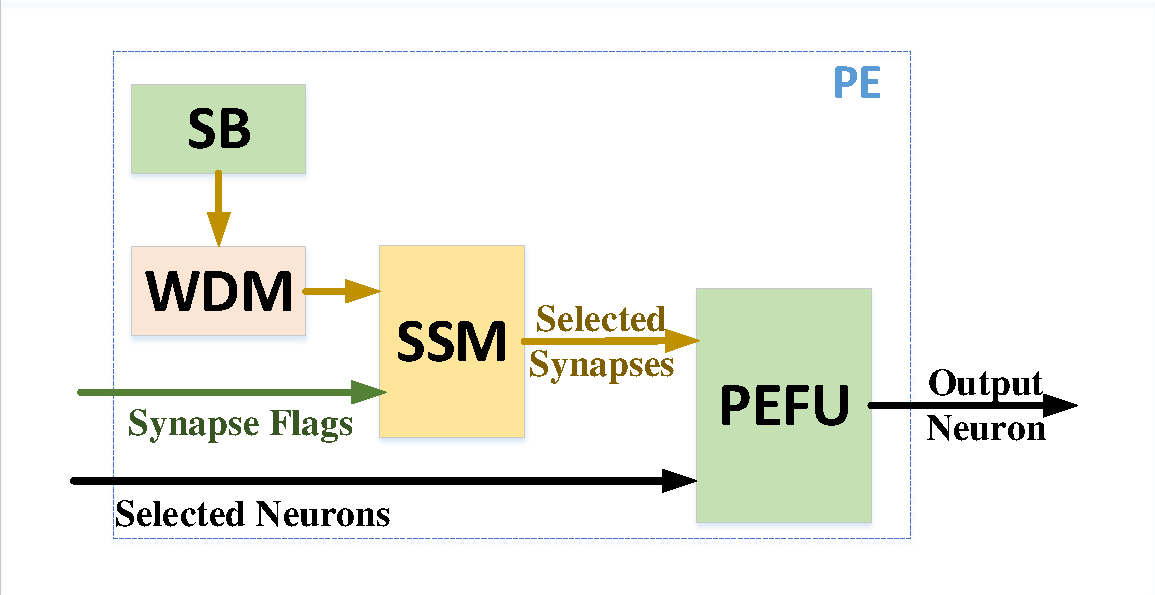
\includegraphics[width=0.8\columnwidth]{PE.pdf}
\caption{PE结构}
\label{fig:PE}
\end{figure}

NFU可以高效地处理神经网络中的所有运算,NFU包含$T_n$个同构的PE来处理动态稀疏性, 同时完成神经网络的运算。如图~\ref{fig:PE}所示,PE由一个局部突触缓存(synapse buffer, SB),权码解码模块(weight decoding module, WDM),突触选择模块(synapse select module, SSM)和处理功能单元(processing element functional unit, PEFU)组成。

\textbf{SB.} SB用来存储PE计算所需要的突触。由于每个PE处理共享相同的输入神经元,但是使用独立的权值计算不同的输出神经元。因此我们在每个PE中集成了一个本地的SB,使得每个PE能够从本地SB中加载权值,从而缓减数据传输中的网络拥塞(network congestion),减少连线开销。

\textbf{WDM.} WDM用来解码经过局部量化的权值。WDM中集成了一个查找表(look-up table, LUT),查找表中存储了权值密码本,查找表的输入为权值字典,最终通过查表操作解码出实际的权值。

\begin{figure}[h]
\centering
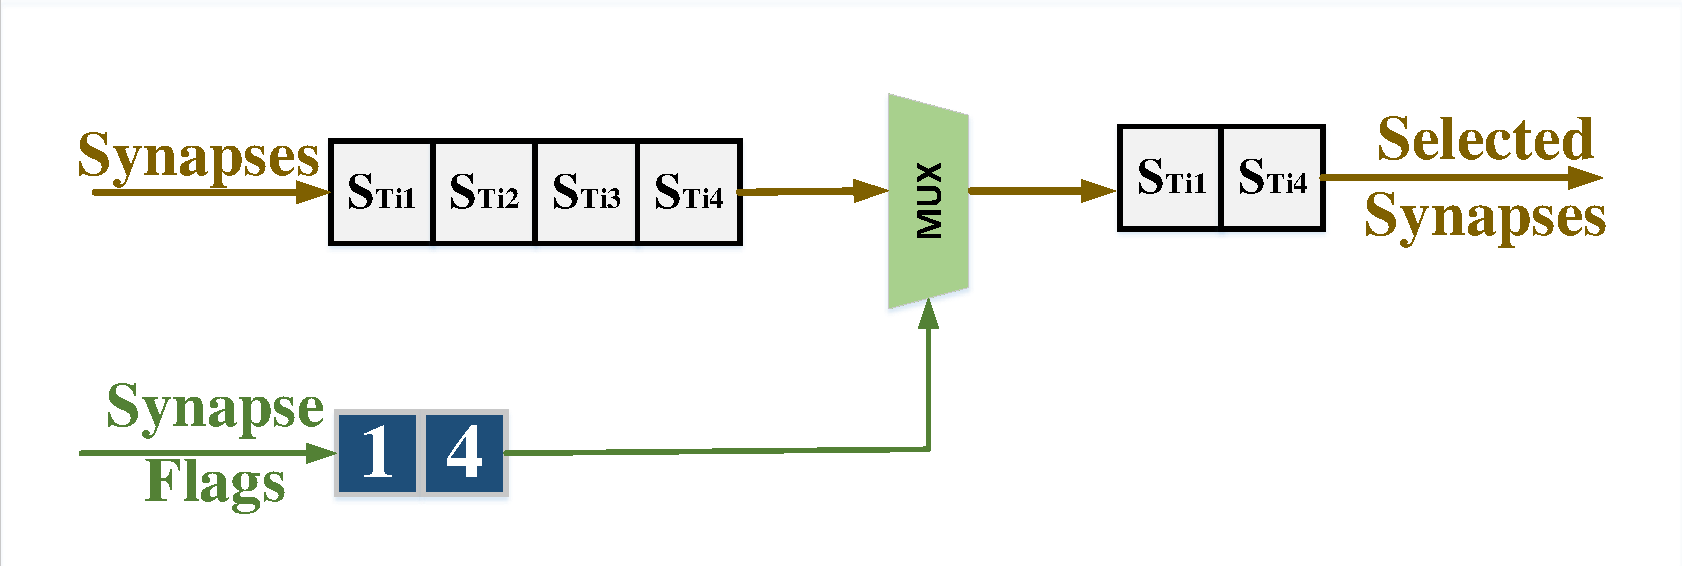
\includegraphics[width=0.8\columnwidth]{SSM.pdf}
\caption{SSM结构}
\label{fig:SSM}
\end{figure}

\textbf{SSM.} \zadd{SSM接收突触和突触标志,处理动态稀疏,最终筛选出需要进行计算的突触(如图~\ref{fig:SSM})。我们利用图~\ref{fig:connection}作为实例来描述SSM筛选突触的流程。在图~\ref{fig:connection}的实例中,对于每个输出神经元$o1, o2, o3$,第一个和第四个突触 ($S_{T_{i}1}$ ,$S_{T_{i}4}$) 是计算所需的两个突触。SSM接收来自NSM的突触标志筛选突触,其中突触标志中包含所需突触位置索引信息(\emph{“14”})。如图~\ref{fig:SSM}所示,SSM在突触与突触标志之间执行 “MUX” 操作,最终筛选出需要进行计算的突触,即$S_{T_{i}1}$ 和$S_{T_{i}4}$。由于每个PE接收不同的突触,并且处理不同的输出神经元,我们在每个PE内部局部集成SSM,从而避免高带宽和长延迟。
}

\begin{figure}[h]
\centering
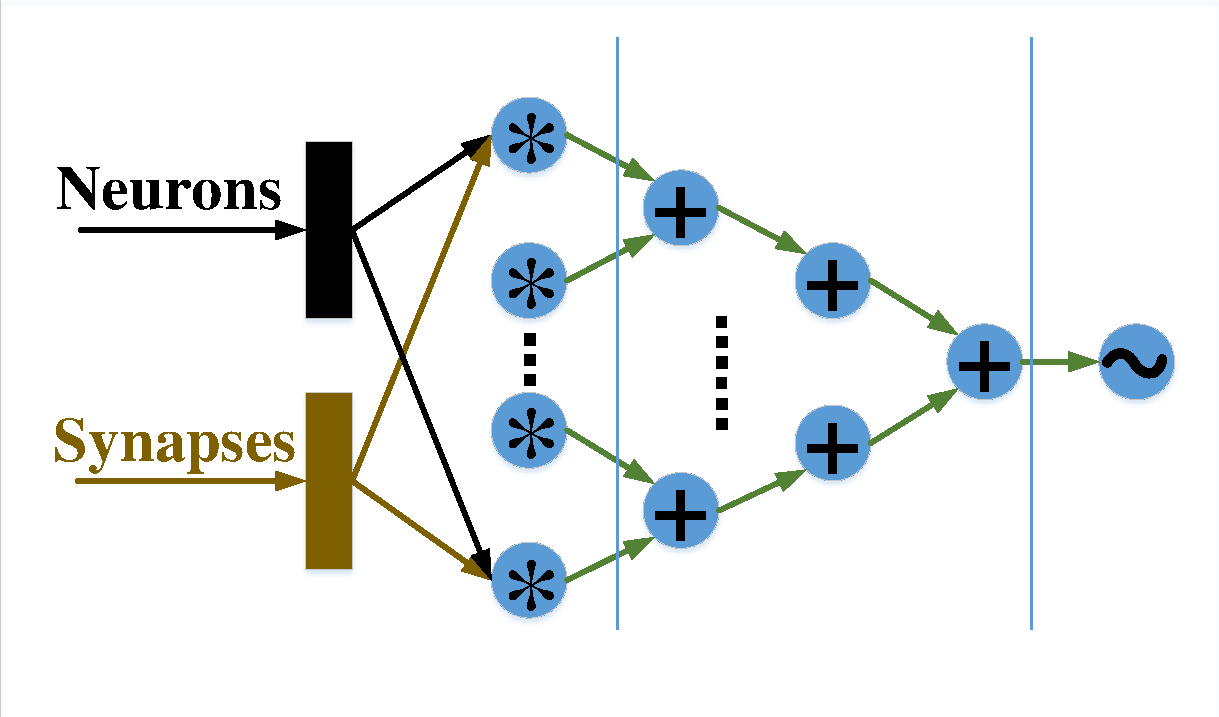
\includegraphics[width=0.8\columnwidth]{PEFU.pdf}
\caption{PEFU结构}
\label{fig:PEFU}
\end{figure}

\textbf{PEFU.} PEFU用来完成神经网络的核心运算。如图~\ref{fig:PEFU}所示,PEFU由三段流水结构,分别完成乘法,累加和非线性的运算。每个PEFU由$T_m$乘法单元,一个$T_m$输入的加法器树和一个非线性函数模块组成。我们使用分时复用的方法将神经网络映射到PE,即每个PE计算一个输出神经元。理想情况下,如果一个输出神经元需要$M$个乘法操作,那么PE需要$\lceil M/T_{m} \rceil$个时钟周期(cycle)完成计算元,因为PEFU可以在一个周期内完成$T_m$次乘法。最后,NFU将从$T_n$个PE中收集$T_n$个输出神经元的部分和,传输到NBout中。 


PEFU中的非线性运算主要是指超越函数(Transcendental Functions)。超越函数是变量之间的关系不能用有限次加、减、乘、除、乘方、开方运算表示的函数。常见的超越函数包括三角函数,指数函数,对数函数,双曲函数等。目前运算超越函数的方法主要有差值查表和迭代两种。其中迭代方法中最有效的方法是CORDIC算法。

CORDIC(Coordinate Rotation Digital Computer)算法即坐标旋转数字计算方法,能够既方便又有效地用来计算三角函数和双曲函数。该算法中涉及到的运算只有加法,减法,移位和查表运算,非常适合用硬件实现。算法由~\citet{Volder1959The}于1959年提出,首先用于导航系统,使得矢量的旋转和定向运算不需要做查三角函数表、乘法、开方及反三角函数等复杂运算。~\citet{Walther1971A}在 1974 年用它研究了一种能计算出多种超越函数的统一算法。CORDIC的每一次迭代能够额外获得1位的精度,因此迭代次数越多,CORDIC的精度也就越高。

线性差值查表的方法目前已经在多个神经网络加速器中被应用~\cite{Temam2012A, chen2014diannao},我们将超越函数分为M个段,对每一段函数使用线性函数进行拟合获得斜率a和截距b,其中第i段可以使用线性函数$f(x) = a_i \times x + b_i$进行近似。

尽管CORDIC的精度高于线性差值查表的方法,但是面积和能耗开销远远高于查表的方法。由于神经网络具有很强的鲁棒性,线性差值查表的方法并不会引起网络精度下降~\cite{Temam2012A},因此我们选择查表的方法完成非线性运算。


\subsubsection{Encoder}
Encoder模块与Nbout直接相连,用于对输出神经元进行压缩,消除输出神经元中的零元素,最终用direct indexing的形式表示稀疏的输出神经元。图~\ref{fig:encoder}展示了神经元压缩模块Encoder的架构。
\zadd{具体来说,Encoder根据神经元的激活值,生成神经元索引(neuron indexes,\emph{“11101010”}),索引中的每一个比特位指示相应的神经元激活是否为零。然后Encoder在神经元与神经元索引之间执行 “MUX” 操作筛选出非零的神经元。最终非零神经元与对应的神经元索引被传输到片外,然后作为下一层网络的输入被重新加载到NBin。通过动态压缩神经元,加速器能够显著减少DRAM访问神经元的开销,从而减少DRAM的访存能耗。
}

\begin{figure}[h]
\centering
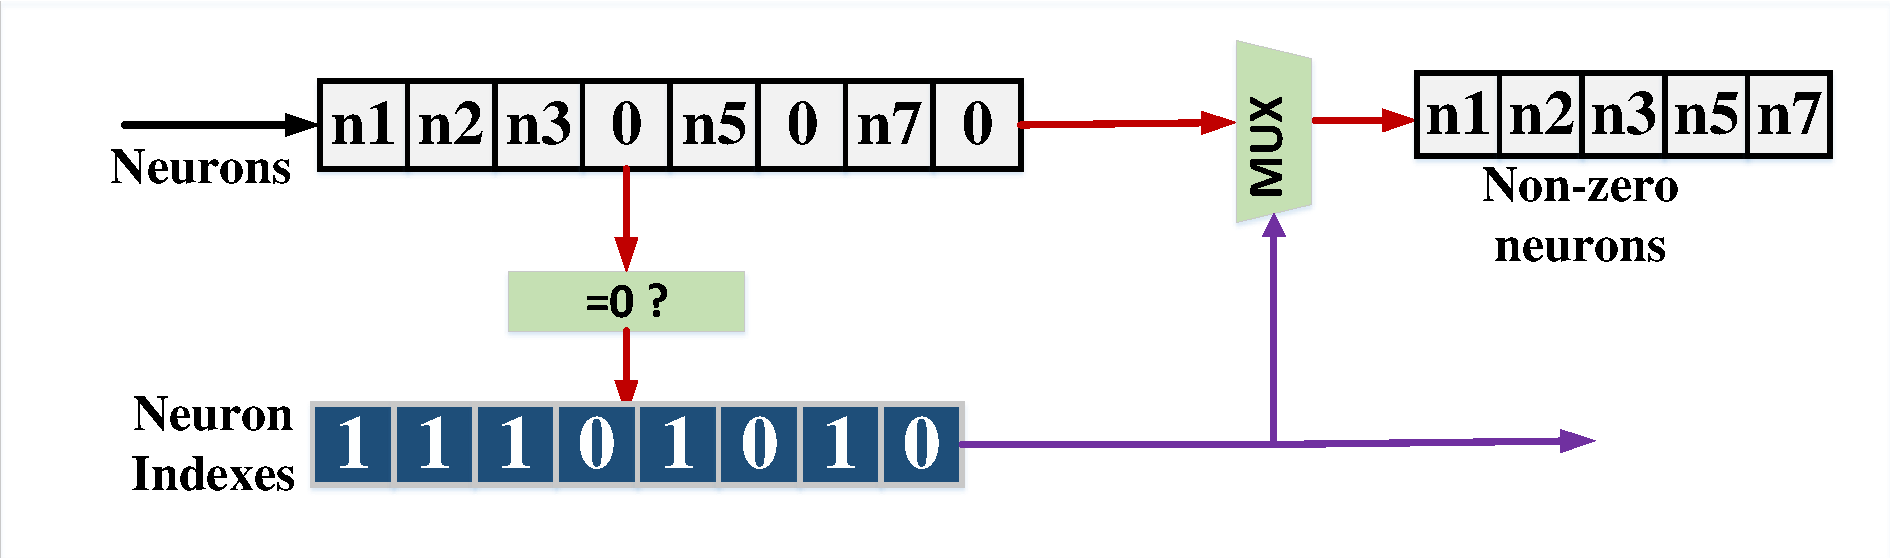
\includegraphics[width=0.8\columnwidth]{encoder.pdf}
\caption{Encoder架构}
\label{fig:encoder}
\end{figure}

\subsection{存储模块}
\label{subsec:storage}

考虑到不同数据在加速器中的不同行为模式,我们将片上缓存分为三个部分:一个输入神经元缓存(NBin),一个输出神经元缓存(NBout)和$T_m$个权值缓存(SB),分别用来存储输入神经元,输出神经元和权值。考虑到神经元稀疏和权值稀疏的情况,我们增加了两个索引缓存,分别是输入神经元索引缓存(NIBin)和权值索引缓存(SIB)。为了实现输出传输与计算之间的重叠(overlap),我们使用乒乓(ping-pong)的模式管理所有的缓存。下面我们将着重讨论各个缓存的带宽和存储容量。

\subsubsection{NBin} 
对于NBin,我们设置带宽为$16\times T_m \times 16$比特,设置这个带宽主要是考虑到PE的利用率。虽然PE共享相同的输入神经元,但是每个PE在一个周期需要$T_m$个输入神经元来避免PEFU中计算单元的空转。考虑到现有大部分神经网络的稠密度都高于$1/16$(即稀疏度低于$15/16$),特别是卷积层,一般稠密度为$30\%$左右,因此,我们在一个周期发送给NSM~~~$16\times T_m$个输入神经元时,就能够保证NSM在一个周期能够筛选出$T_m$个输入神经元,从而保证PEFU的运行效率。

\subsubsection{NBout} 
对于NBout,我们设置其带宽为$4\times T_n \times 16$比特,这部分主要是考虑到动态神经元稀疏。如表~\ref{tab:sparsities}考虑到现有大部分神经网络的神经元稠密度高于$25\%$(即稀疏度低于$75\%$),当我们在每一个周期发送给Encoder~~~$4\times T_n$个输出神经元时,就能够保证Encoder在一个周期筛选出$T_n$个神经元进行压缩,从而充分利用NBout与片外DDR之间的带宽。

\subsubsection{SB}
对于每一个PE中的SB,我们设置带宽$4\times T_m\times 16$比特,保证能够在一个周期读取$4\times T_m$个权值。考虑到现有大部分神经网络的动态稀疏度低于$75\%$,$4\times T_m \times 16$比特的带宽能够保证SSM在一个周期筛选出$T_m$个权值,从而保证PEFU的运行效率。由于权值是以压缩形式(通过剪枝和局部量化)存储在SB中,局部量化会导致权值在不同的神经网络和不同层中的位宽不同,例如,在AlexNet网络的卷积层中权值被量化为8比特,在MLP网络的全连接层中权值被量化为6比特,在AlexNet网络的全连接层中权值被量化为4比特。不同的量化比特会导致WDM模块庞大的面积/功耗开销,因此我们将权值按照4比特进行对齐操作。例如,假设SRAM的一行为128比特,那么当权值被量化为16比特,8比特和4比特时,SRAM的一行分别能够存储8个,16个和32个权值。因此,$T_m \times 64$比特的权值能够被WDM解码成为$T_m \times 16$个权值(当权值被编码成小于或者等于4比特),或者$T_m \times 8$个权值(当权值被编码成大于4比特而小于等于8比特),或者$T_m \time 4$个权值(当权值被编码成大于8比特,小于等于16比特)。对比于支持所有位宽编码形式的解码模块,我们的WDM能够减少5.14倍的面积和4.27的功耗。

\subsubsection{NIBin和SIB}
对于NIBin和SIB,我们设定其宽度为$16\times T_m\times 1$比特,因为我们使用直接索引的方式存储稀疏的神经元和权值,索引中的每一比特用于表示对应的元素是否为“0”。因此,NIBin和SIB则需要$16\times T_m\times 1$比特的带宽与Nbin提供给NSM的$16\times T_m$个输入神经元一一对应。

\subsubsection{缓存大小}
五个缓存的大小决定了整个架构的整体性能和能耗。尽管有部分研究~\cite{chen2014dadiannao,han2016eie}提出,加速器需要提供足够大的缓存来保存神经网络所有的权值和神经元从而避免高昂的片外访存开销,但是这种设计会大大增加延迟,面积,功耗;同时这种设计方案缺少可扩展性,并不能很好地支持新兴的规模更大,层数更深的神经网络。因此我们使用小的缓存以及适当的数据替换策略,将数据分多次传输到片上进行运算,从而权衡加速器的可扩展性,性能和能耗。在探索了不同大小的缓存区后,我们设定NBin,NBout,SB,SINin和SIB的大小分别是$8KB$,$8KB$,$32KB$,$1KB$和$1KB$。

\subsection{控制}
\label{subsec:control}

CP用于控制加速器的整个执行流程。它从内部指令缓存中读取指令然后进行解码,从而有效地协调数据摆放形式,内存访问和数据计算的过程。CP通过监控各个模块对应的状态寄存器来监控每个模块的状态,然后通过设置各个模块的控制寄存器管理各个模块的运行。我们利用基于库的编译器生成高效的超长指令字(Very Long Instruction Word,VLIW)。

\subsubsection{状态机}
我们为CP设计了高效的有限状态机(finite state machine, FSM)。如图~\ref{fig:FSM}所示,FSM分为两层控制状态,第一层状态表示神经网络中的宏观操作,如卷积,内积,池化,激活等操作;第二层状态则是每一个宏观操作中的细节,如对于卷积操作还会有数据预取,计算,写回等不同的状态。分层有限状态自动机能够限制状态机的跳转,从而简化状态机的设计。

\begin{figure}[h]
\centering
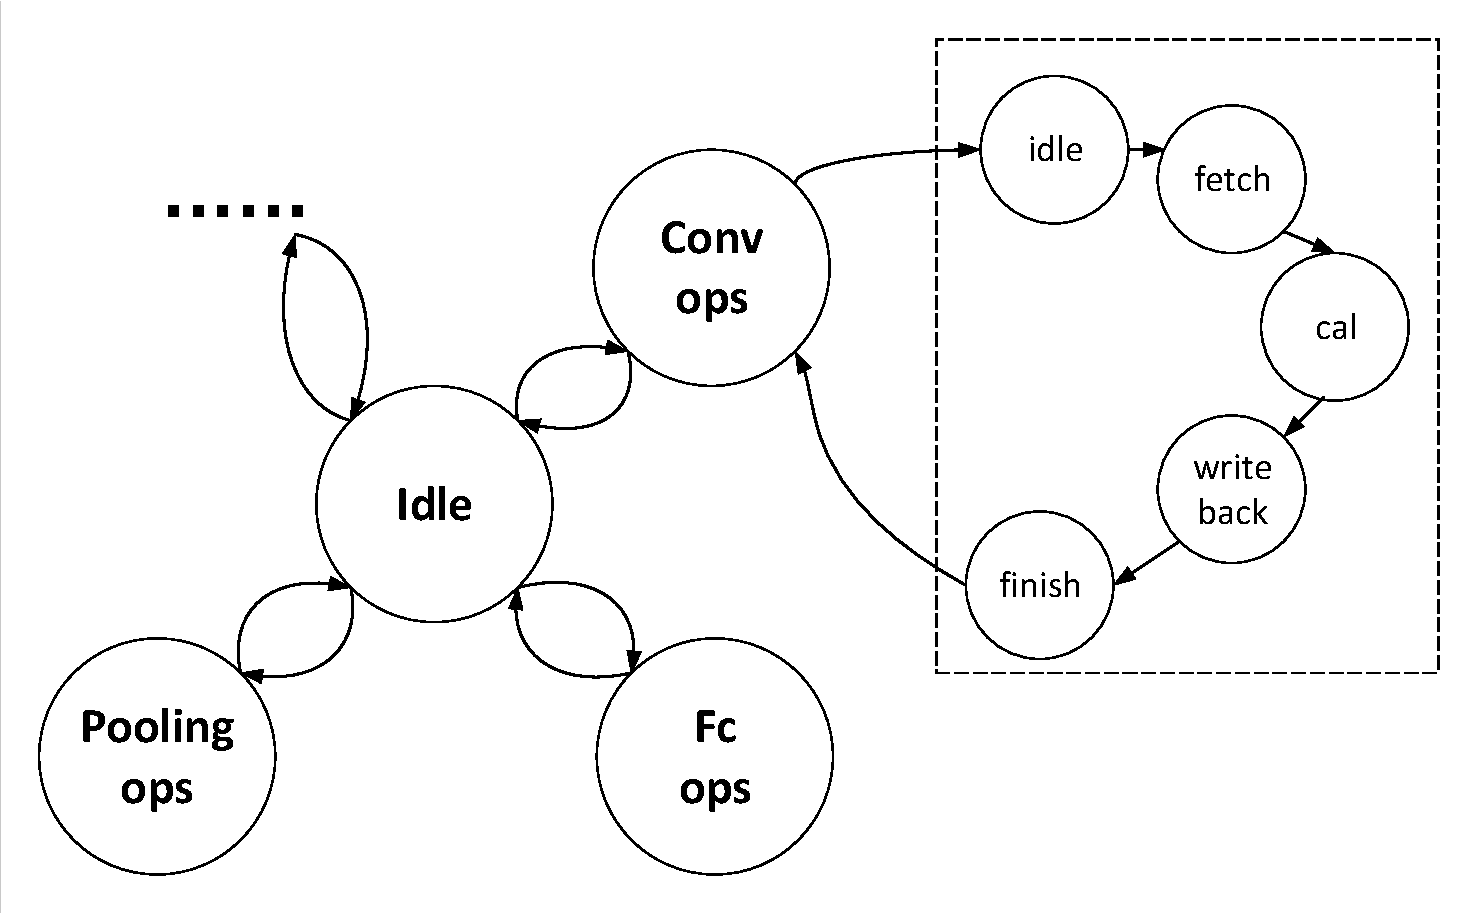
\includegraphics[width=0.8\columnwidth]{FSM.pdf}
\caption{CP的有限状态机}
\label{fig:FSM}
\end{figure}

\subsubsection{多发射控制器}
单指令发射的控制器会忽视一些潜在的提高加速器性能的因素。单发射的控制器需要等待IO指令(Load/Store)将数据完全从片外搬运到片上缓存后才能发射下一条计算指令,即使我们采用乒乓的方式管理片上缓存也无法使IO指令和计算指令并行执行。一种简单但是有效的解决方案是加速器的控制器能够提前解码下一条指令,如果不与上一条指令不冲突,则发射下一条指令。因此,我们设计了一个多发射控制器,用于充分挖掘IO指令与计算指令之间的并行性。

多发射控制器的关键特征是能够在一个周期内发射多条没有依赖关系的指令。一般来说,没有依赖关系的指令包括三个方面,首先IO指令与计算指令之间没有依赖关系,可以同时发射执行;第二,由于Off-chip Memory和片上SRAM均采用双端口的设计模式,因此Load和Store指令之间没有依赖关系,可以同时发射执行;第三,如果计算指令涉及不同的计算单元和数据,那么这些计算指令也能同时发射执行。IO指令主要包括NBin、SB以及NBout与片外之间的Load/Store指令;计算指令主要包括矩阵、向量、标量,逻辑运算等。我们在编译过程中静态分析指令之间的依赖关系,提取出没有相互依赖关系的指令,在执行时同时进行发射。由于多发射控制器在一个周期需要解码/发射多条指令,我们需要为指令缓存(IB)设计更高的带宽,使其能在一个周期为多发射控制器提供多条指令。

\subsection{片上互联}


如图~\ref{fig:Htree}所示,我们采用H树的拓扑结构连接NSM与NFU中的$T_n$个PE。由于NSM筛选产生的神经元和突触标志被所有PE共享,而且PE之间的负载是一种均衡的状态,因此NSM通过H树将这些信息通过广播的形式传送给PE,从而避免NSM和PE之间由于距离差异引起的不平衡延迟的问题;同时H树拥有非常良好的可扩展性,能够非常方便地对PE进行扩展,在不改变整体拓扑结构的情况下通过增加PE的数量增加加速器的计算能力,从而应对更大规模的神经网络。

\begin{figure}[h]
\centering
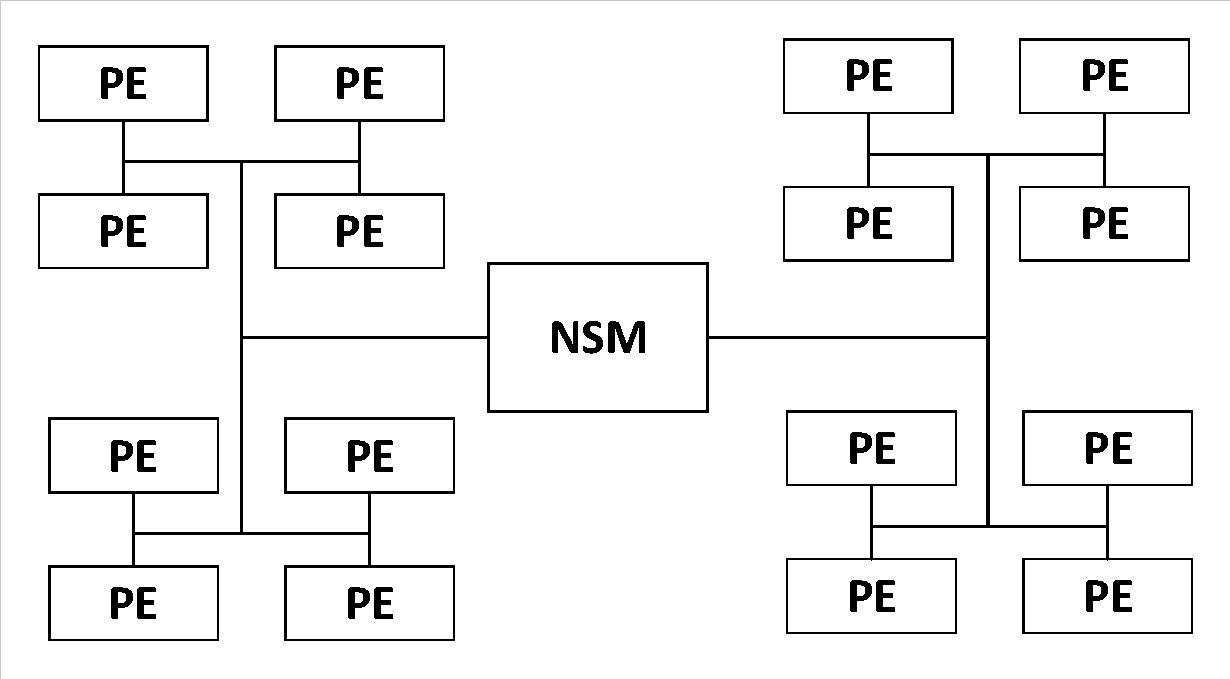
\includegraphics[width=0.8\columnwidth]{Htree.pdf}
\caption{H树互联结构}
\label{fig:Htree}
\end{figure}

\section{编程模型}

\subsection{基于库的编程模型}
考虑到实际应用场景和开发效率,高级编程模型(如Caffe~\cite{jia2014caffe}、Tensorflow~\cite{abadi2016tensorflow}、MXNet~\cite{chen2015mxnet}等)为用户提供了一系列C++的库函数接口,使得用户能够方便地调用这些接口,从而控制CPU或者GPU完成神经网络的运算。高级编程模型能够大幅度增加用户或者开发人员的编程效率,特别是算法和应用程序开发人员。因此,专用的加速器必须为用户提供类似于高级编程框架的接口,以减轻用户的编程负担。为此,我们提供了基于库的编程模型,其基本思想是为用户提供一系列C++的高级库函数接口,每一个函数对应了神经网络中一个基本操作,如卷积运算,内积,池化等操作。

代码~\ref{list:conv}是卷积层库函数的接口,卷积库接口分为两部分,分别是数据定义和操作定义。用户首先通过TensorDescriptor和FilterDescriptor定义卷积操作所涉及输入/输出和权值;同时分别使用setTensorDescriptor和setFilterDescriptor分别描述输入/输出和权值的特性,如稀疏、规模、地址等。然后用户通过ConvDescriptor和setConvDescriptor分别定义卷积操作描述符和卷积操作的特性,如输入/输入/权值规模,步长,补白(padding)等。最后用户调用convForward执行卷积操作。用户通过调用这个库函数接口能够非常方便地最终驱动加速器完成卷积操作。

\newpage

\begin{lstlisting}[language=C, frame=single, basicstyle=\footnotesize, caption=卷积层库函数接口, label=list:conv, captionpos=b]
  // Data Declaration
  TensorDescriptor input, output;
  FilterDescriptor weight;
  setTensorDescriptor(input, ...);
  setTensorDescriptor(output, ...);
  setFilterDescriptor(weight, ...);
  // Operations
  ConvDescriptor conv;
  setConvDescriptor(...);
  ConvForward(conv, input, weight, output);
\end{lstlisting}

我们将库嵌入到深度学习框架Caffe中,如图~\ref{fig:framework}所示,这一套编程框架对用户完全透明,使得用户能够无缝使用加速器。值得注意的是我们需要为Cambricon-S设计专用的编译器(compiler),使其能够将C++源码编译成为加速器中的可执行指令。

\begin{figure}[ht]
\centering
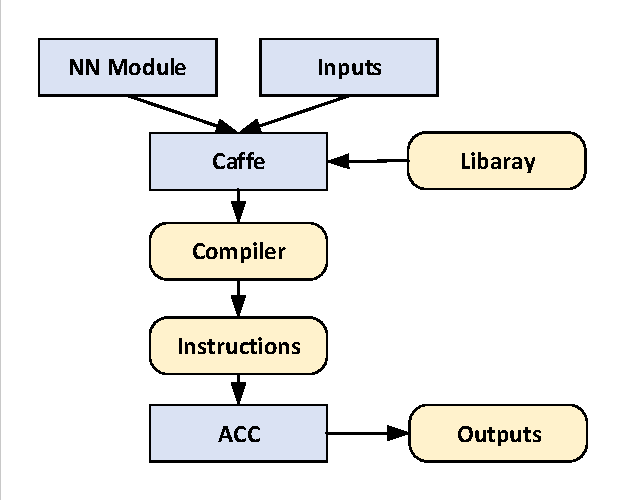
\includegraphics[width=0.7\columnwidth]{framework.pdf}
\caption{编程框架}
\label{fig:framework}
\end{figure}

\subsection{编译器}
深度学习框架(如caffe)与加速器之间存在巨大的鸿沟,如何为加速器建立一套完整的编程生态系统是一个巨大的挑战。为此我们需要为加速器设计专用的基于库的编译器,从而将基于库的源文件编译成为加速器中可执行指令。编译的主要挑战来源于加速器中复杂的片上数据管理。

具体来说,第一,神经网络中的数据多样性和特征多样性增加了数据分配和数据搬运的复杂度。由于神经网络中有不同类型的参数,如输入/输出神经元,权值等;同时不同的数据拥有不同的特征,如神经元有动态稀疏的特性,权值有静态稀疏和量化的特性。如何根据数据的特征为不同的数据种类分配数据空间,如何搬运不同种类的数据成为一个巨大挑战,因此,我们为不同的数据使用适当的数据分配和数据搬运策略来提升效率。

第二,有限的片上缓存增大了数据调度的复杂性。考虑到神经网络中庞大的神经元/突触的和加速器中有限的片上内存之间的矛盾,我们需要使用循环分块(loop tiling)对数据进行切分,同时使用合适的数据重用策略提升加速器的性能。而不同的循环分块策略和数据重用 (data reuse) 策略会进一步影响片外数据访问,片上数据访问,计算调度,从而影响加速器的效率和性能。因此我们需要在编译期间探索不同的循环分块策略和数据复用策略,选择最优的循环分块方式和最佳的数据重用策略,最大程度挖掘加速器的性能。

\begin{figure}[h]

\centering
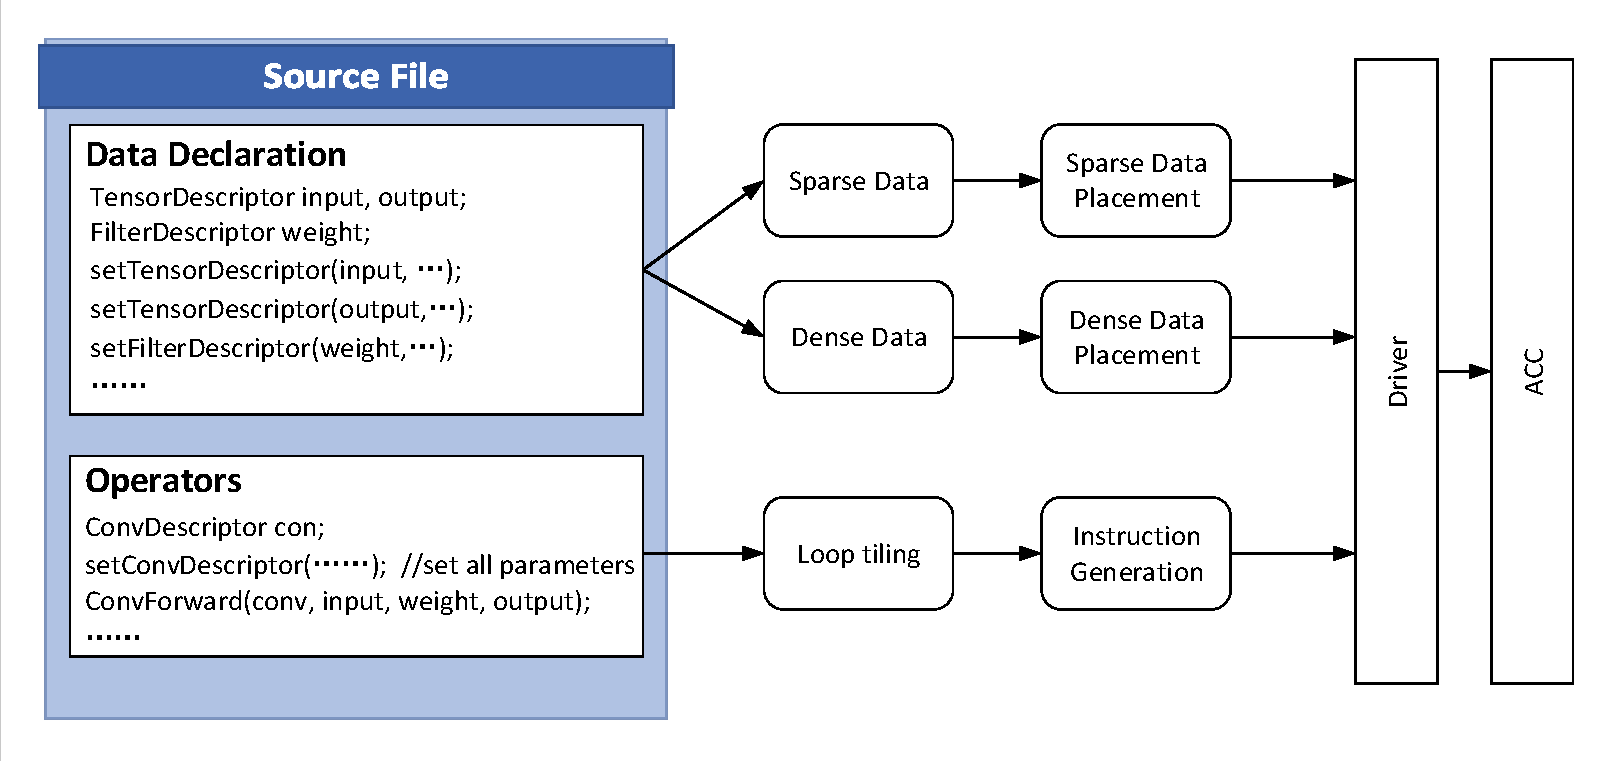
\includegraphics[width=0.8\columnwidth]{compiler.pdf}
\caption{源文件编译成为加速器可执行代码的过程}
\label{fig:compiler}
\end{figure}

我们为加速器设计了一个专用的编译器来弥合深度学习框架与加速器之间的差距。如图~\ref{fig:compiler}所示,我们显示了如何将基于库的源文件编译成为加速器的可执行代码。编译过程分为两个阶段:数据摆放(data placement)和指令生成(instruction generation)。

在数据摆放阶段,源代码中的数据结构被合理地分配到加速器的片上缓存中。我们使用张量(tensor)对输入和输出神经元进行封装,同时我们用过滤器(filter)对权值进行封装,值得注意的是,tensor和filter都是四维的张量。我们使用不同的数据结构封装不同数据类型,是因为不同类型的数据会被分配到加速器不同的片上缓存中(如输入神经元,输出神经元和权值会分别被分配到NBin,NBout和SB中)。同时考虑到数据稀疏的特性,我们使用sparse这个枚举类型作为描述符,并将其添加到tensor(动态神经元稀疏)和filter(静态权值稀疏)的属性中。

在指令生成阶段,考虑到有限的片上缓存,我们需要使用循环分块将运算操作(包括卷积操作,池化操作等)分解为子操作,以确保子操作对应的数据能够(即输入/输出神经元,权值)能够填充到有限的片上缓存中。值得注意的是,运算操作对应的IO操作和访存操作会被同时生成。最终指令生成器将这些操作转换为对应的运算指令,IO指令和访存指令。更进一步的,指令生成器会对生成的指令进行静态依赖分析,提取出没有依赖关系的指令并进行标记,在这个过程中,指令生成器主要关注IO指令与计算指令之间的依赖关系,Load/Store指令之间的依赖关系,以及不同计算单元对应的计算指令之间的依赖关系。最终,指令生成器生成加速器可以解码和执行的指令,同时没有依赖关系的指令可以同时发射执行。

\subsection{循环分块}

循环分块(loop tiling)能够对计算进行合理划分,以确保子计算所涉及的数据能够被完全填充到片上缓存中。由于片外访存会花费巨大的能耗(占用超过$90\%$的整体能耗),因此循环分块策略优先考虑如何提高片上数据重用性,从而减少片外数据访存,从而减少加速器的访存能耗。Eyeriss~\cite{chen2017eyeriss}提出了四种不同的数据重用策略,分别是卷积重用(\emph{convolutional reuse}),卷积核重用(\emph{filter reuse}),输入特征图重用(\emph{input feature map reuse})和部分和重用(\emph{partial sums reuse})。考虑到Cambricon-S与Eyeriss架构上的差异,我们将数据重用策略分为三种类型,即输出重用(\emph{output-reuse}, 与Eyeriss中的\emph{partial sums reuse}对应),突触重用(\emph{synapse-reuse},与Eyeriss中的\emph{convolutional reuse}和\emph{filter reuse}对应)和输入重用(\emph{input-reuse},与Eyeriss中\emph{input feature map resue}对应);这三种策略分别表示最大程度重用输出数据,突触数据和输入数据。

对于输出重用策略,在运算过程中,一段输入神经元被加载到NBin中,一段权值被加载到SB中,然后计算出一段输出神经元的部分和,并将其存储到NBout中;在下一个阶段,第二段的输入神经元和权值被加载到片上缓存持续计算NBout中输出神经元部分和,这个过程一直循环直至NBout中的这一段输出神经元被完全计算完成,最后NBout中的输出神经元被存储到片外;因此在输出重用策略中,输入神经元和权值会多次从片外加载到片上缓存,而输出神经元部分和会持续存储在NBout中直至被完全计算完成。同理,在突触重用策略中,输入神经元和输出神经元部分和会被多次从片外加载到片上,直至片上的权值被完全重用。在输入重用策略中,权值和输出神经元部分和会被多次从片外加载到片上,直至片上的输入神经元被完全重用。因此我们在编译阶段需要探索最佳的数据重用策略,减少片外访存的能耗。

不失一般性的,我们以VGG16网络的\emph{conv4\_2}卷积层为例,来计算不同的数据重用策略对片外访存的需求。具体来说,\emph{conv4\_2}的输入规模为$30\times 30\times 512$(考虑到输入需要进行补白),权值的规模为$32\times 32\times 512\times 512$, 输出的规模为$28\times 28\times 512$,其中输入神经元和权值的稠密度分别是$40.52\%$(稀疏度为$59.48\%$)和$34.20\%$(稀疏度为$65.80\%$)(如表~\ref{tab:sparsities}所示),权值和神经元均为16比特定点。加速器中NBin,SB和NBout的大小分别是$8KB$,$32KB$和$8KB$。在循环分块过程中,我们将数据且分为$SegN$块,其中每一块数据量为$SegSize$。为了尽可能提高片上缓存的利用率,我们将输出的$C$维度按照$4\times 128$($SegN\times SegSize$)的方式进行切分,在$H$维度按照$28\times 1$的方式进行切分;同时我们将输入的$C$方向按照$16\times 32$的方式进行切分。经过循环分块后,输入、权值、输出d的每一个数据块的大小分别为$SegSize_{in} = 30\times 3\times 32\times 40.52\%$, $SegSize_{syn} = 3\times 3\times 32\times 128\times 34.20\%$ 和 $SegSize_{out} = 28\times 1\times 128$。值得注意的是,我们对输入数据块和权值数据块分别乘以网络的稠密度来进行近似。因此,使用输入重用,输出重用和突触重用策略,所需要的片外访存的开销可以按照如下公式进行计算:

\begin{align*}
MEM_{i} & = 16 \times 1 \times 28 \times (SegSize_{in} + SegSize_{syn} \times 4 + SegSize_{out} \times 4 \times 2)\times 2 \\
      & = 68.59MB \\
MEM_{o} & = 4 \times 28 \times 1 \times (SegSize_{out} + SegSize_{in} \times 16 + SegSize_{syn} \times 16)\times 2 \\
      & = 47.85MB \\
MEM_{s} & = 16 \times 4 \times (SegSize_{syn} + SegSize_{in} \times 28 \times 1 + SegSize_{out} \times 28 \times 2)\times 2 \\
      & = 30.03MB 
\end{align*}

最终,输入重用、输出重用和突触重用策略需要的片外访存量分别是$69.59MB$、$47.85MB$和$30.03MB$,因此我们在~\emph{conv4\_2}卷积层上选择突触重用的策略。

\section{本章小结}
\zadd{本章我们提出了一个粗粒度稀疏神经网络加速器Cambricon-S。该加速器能充分挖掘深度压缩神经网络的特性,包括粗粒度稀疏和局部量化。}

\zadd{我们首先充分分析粗粒度稀疏神经网络的特性,提出对应的设计原则来指导加速器的设计。我们发现,在粗粒度稀疏神经网络中,多个输出神经元能够共享输入神经元和突触索引,同时多个输出神经元之间负载均衡。这些特性能够大大简化加速器的设计复杂度。}

\zadd{基于粗粒度稀疏神经网络的特性,我们提出了Cambricon-S微结构。该微结构最主要的特征是稀疏处理模块,包括NSM,SSM,Encoder和WDM,分别用来处理粗粒度权值稀疏,处理动态神经元稀疏,动态压缩神经元和解码经过量化的权值。为了充分挖掘计算和访存之间的并行性,提升加速器的性能,我们设计了一个多发射的控制器,能够同时发射多条没有依赖关系的指令。}

\zadd{更进一步的,我们为加速器设计了专用的基于库的编程模型,减轻用户的编程负担。
编程模型中集成了加速器专用的编译器,能够将C++高级语言编译成为加速器可执行指令;值得注意的,编译器能够静态分析指令之间的依赖关系,提取出没有依赖关系的指令,使它们能够在加速器中同时进行发射。
}

